\pdfminorversion=4
\documentclass[aspectratio=169]{beamer}

\mode<presentation>
{
  \usetheme{default}
  \usecolortheme{default}
  \usefonttheme{default}
  \setbeamertemplate{navigation symbols}{}
  \setbeamertemplate{caption}[numbered]
  \setbeamertemplate{footline}[frame number]  % or "page number"
  \setbeamercolor{frametitle}{fg=white}
  \setbeamercolor{footline}{fg=black}
} 

\usepackage[english]{babel}
\usepackage[utf8x]{inputenc}
\usepackage{tikz}
\usepackage{courier}
\usepackage{array}
\usepackage{bold-extra}
\usepackage{minted}
\usepackage[thicklines]{cancel}
\usepackage{fancyvrb}

\xdefinecolor{dianablue}{rgb}{0.18,0.24,0.31}
\xdefinecolor{darkblue}{rgb}{0.1,0.1,0.7}
\xdefinecolor{darkgreen}{rgb}{0,0.5,0}
\xdefinecolor{darkgrey}{rgb}{0.35,0.35,0.35}
\xdefinecolor{darkorange}{rgb}{0.8,0.5,0}
\xdefinecolor{darkred}{rgb}{0.7,0,0}
\definecolor{darkgreen}{rgb}{0,0.6,0}
\definecolor{mauve}{rgb}{0.58,0,0.82}

\title[2021-12-06-uvirginia-hep-languages]{Programming Languages, Toolkits, and Communities \\ in Particle Physics Data Analysis}
\author{Jim Pivarski}
\institute{Princeton University -- IRIS-HEP}
\date{December 6, 2021}

\usetikzlibrary{shapes.callouts}

\begin{document}

\logo{\pgfputat{\pgfxy(0.11, 7.4)}{\pgfbox[right,base]{\tikz{\filldraw[fill=dianablue, draw=none] (0 cm, 0 cm) rectangle (50 cm, 1 cm);}\mbox{\hspace{-8 cm}
\includegraphics[height=1 cm]{princeton-logo-long.png}\hspace{0.1 cm}\raisebox{0.1 cm}{
\includegraphics[height=0.8 cm]{iris-hep-logo-long.png}}\hspace{0.1 cm}}}}}

\begin{frame}
  \titlepage
\end{frame}

\logo{\pgfputat{\pgfxy(0.11, 7.4)}{\pgfbox[right,base]{\tikz{\filldraw[fill=dianablue, draw=none] (0 cm, 0 cm) rectangle (50 cm, 1 cm);}\mbox{\hspace{-8 cm}
\includegraphics[height=1 cm]{princeton-logo.png}\hspace{0.1 cm}\raisebox{0.1 cm}{
\includegraphics[height=0.8 cm]{iris-hep-logo.png}}\hspace{0.1 cm}}}}}

% Uncomment these lines for an automatically generated outline.
%\begin{frame}{Outline}
%  \tableofcontents
%\end{frame}

% START START START START START START START START START START START START START

\begin{frame}{Very rough outline of this talk}
\vspace{0.15 cm}
\begin{columns}
\column{1.15\linewidth}
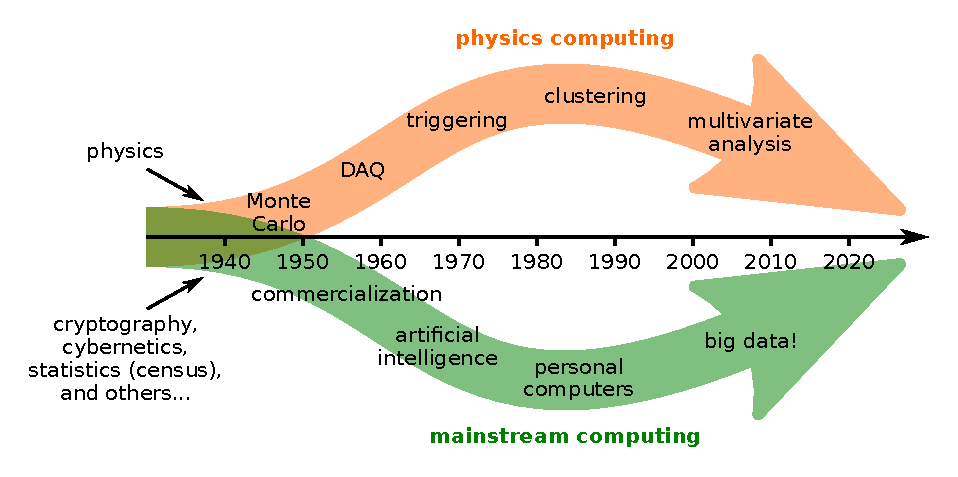
\includegraphics[width=\linewidth]{PLOTS/grand-timeline.pdf}
\end{columns}
\end{frame}

\begin{frame}{\mbox{ }}
\LARGE
\begin{center}
\textcolor{darkblue}{Physicists were involved in (some of) \\ the earliest computers}
\end{center}
\end{frame}

\begin{frame}{Not these\ldots}
\vspace{0.5 cm}

\begin{columns}
\column{0.5\linewidth}
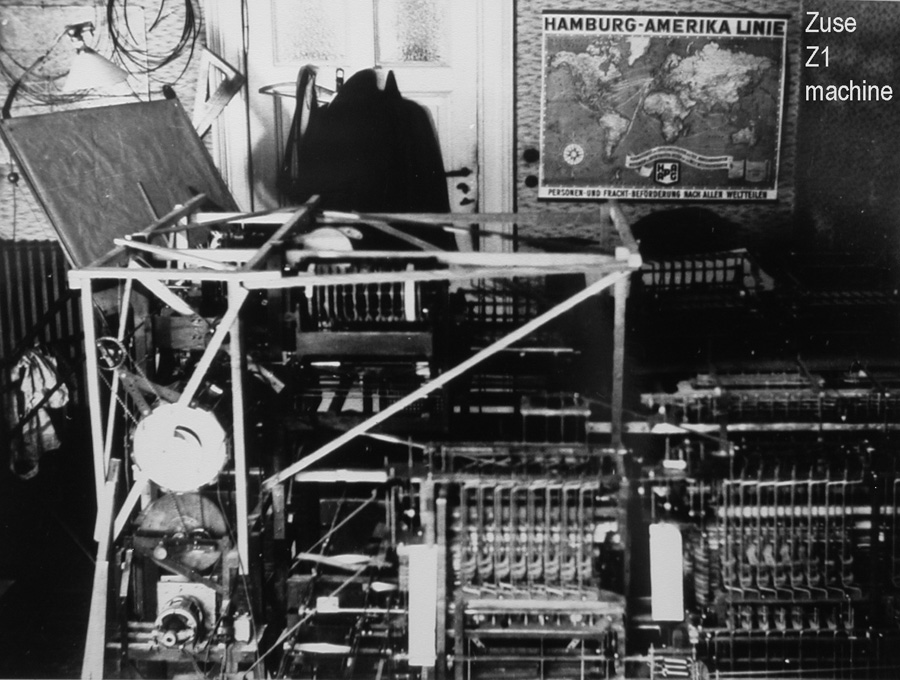
\includegraphics[width=\linewidth]{PLOTS/zuse-z1-living-room.jpg}
\column{0.5\linewidth}
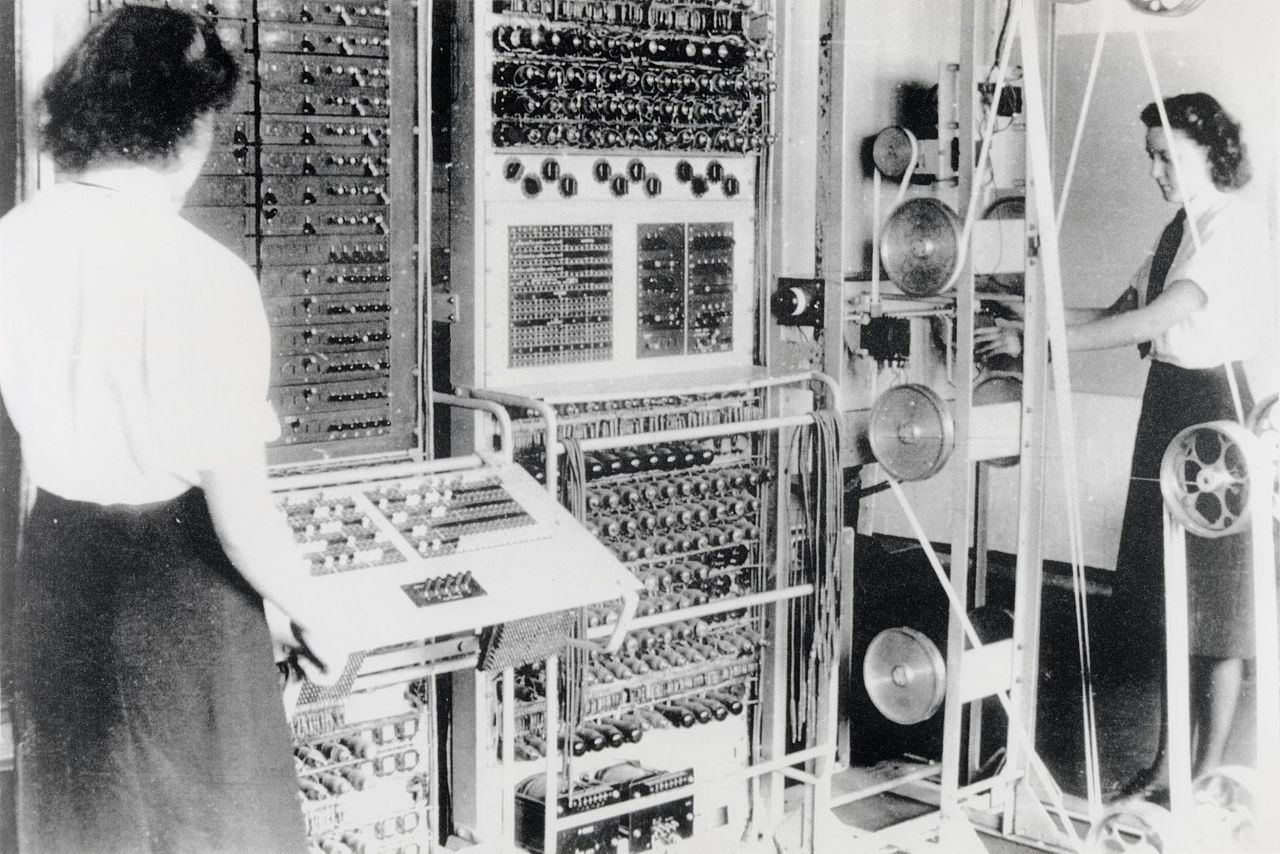
\includegraphics[width=\linewidth]{PLOTS/dorothy-du-boisson-AND-elsie-booker-COLOSSUS-MARK2.jpg}
\end{columns}

\vspace{0.5 cm}
\begin{columns}[t]
\column{0.5\linewidth}
Konrad Zuse's Z1 computer, built in his parents' living room in Berlin in 1937 (destroyed with all blueprints in 1943).

\column{0.5\linewidth}
Colossus Mark 2, operated by Dorothy Du Boisson and Elsie Booker at Britain's codebreaking lab in 1943.
\end{columns}
\end{frame}

\begin{frame}{But this one: ENIAC, the first widely-known computer (1945)}
\vspace{0.35 cm}

\mbox{\hspace{-0.25 cm}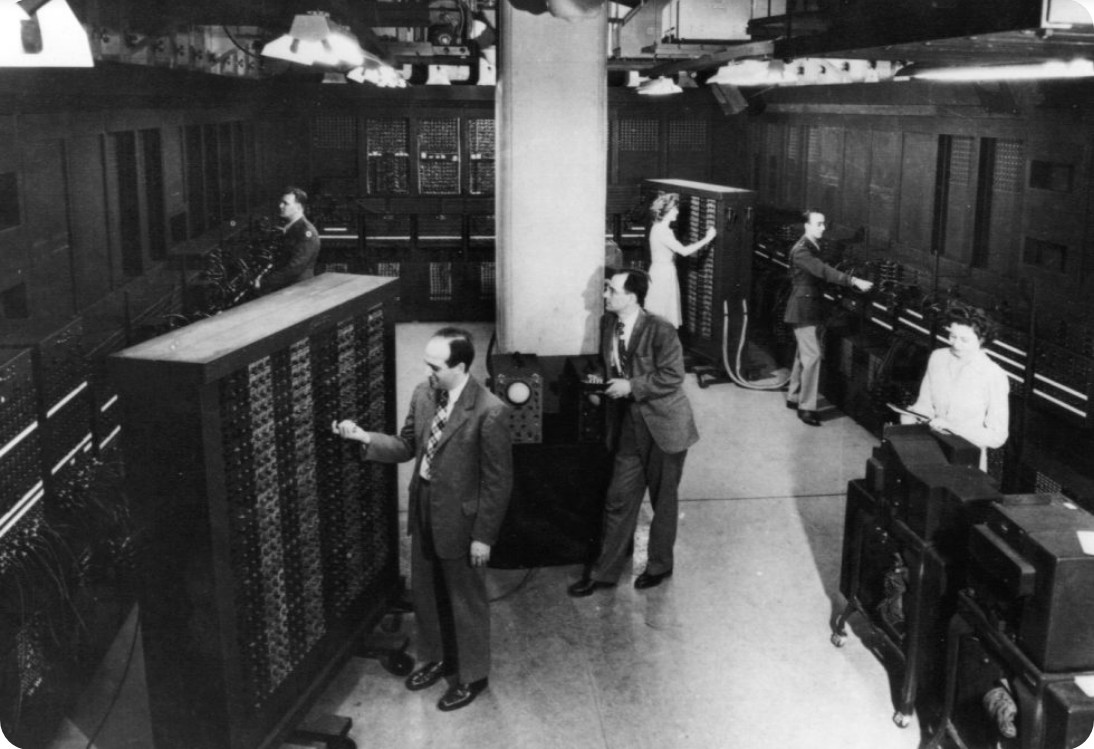
\includegraphics[height=7.5 cm]{PLOTS/eniac-1.jpg}}

\begin{onlyenv}<2->
\vspace{-7.5 cm}
\mbox{\hspace{0.75 cm}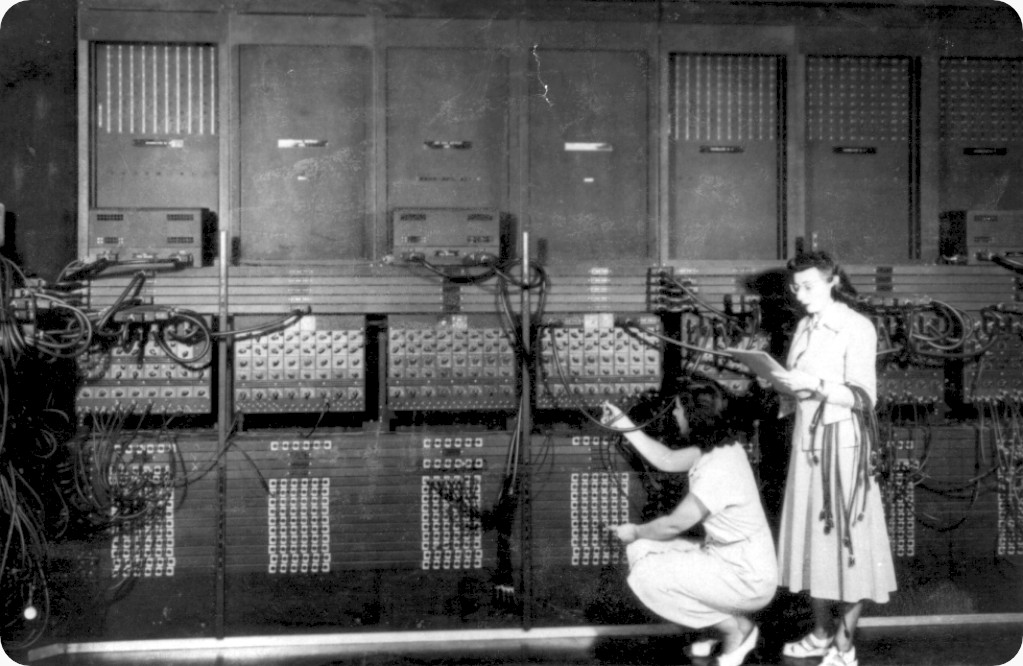
\includegraphics[height=7.5 cm]{PLOTS/eniac-2.jpg}}
\end{onlyenv}

\begin{onlyenv}<3->
\vspace{-7.5 cm}
\mbox{\hspace{1.75 cm}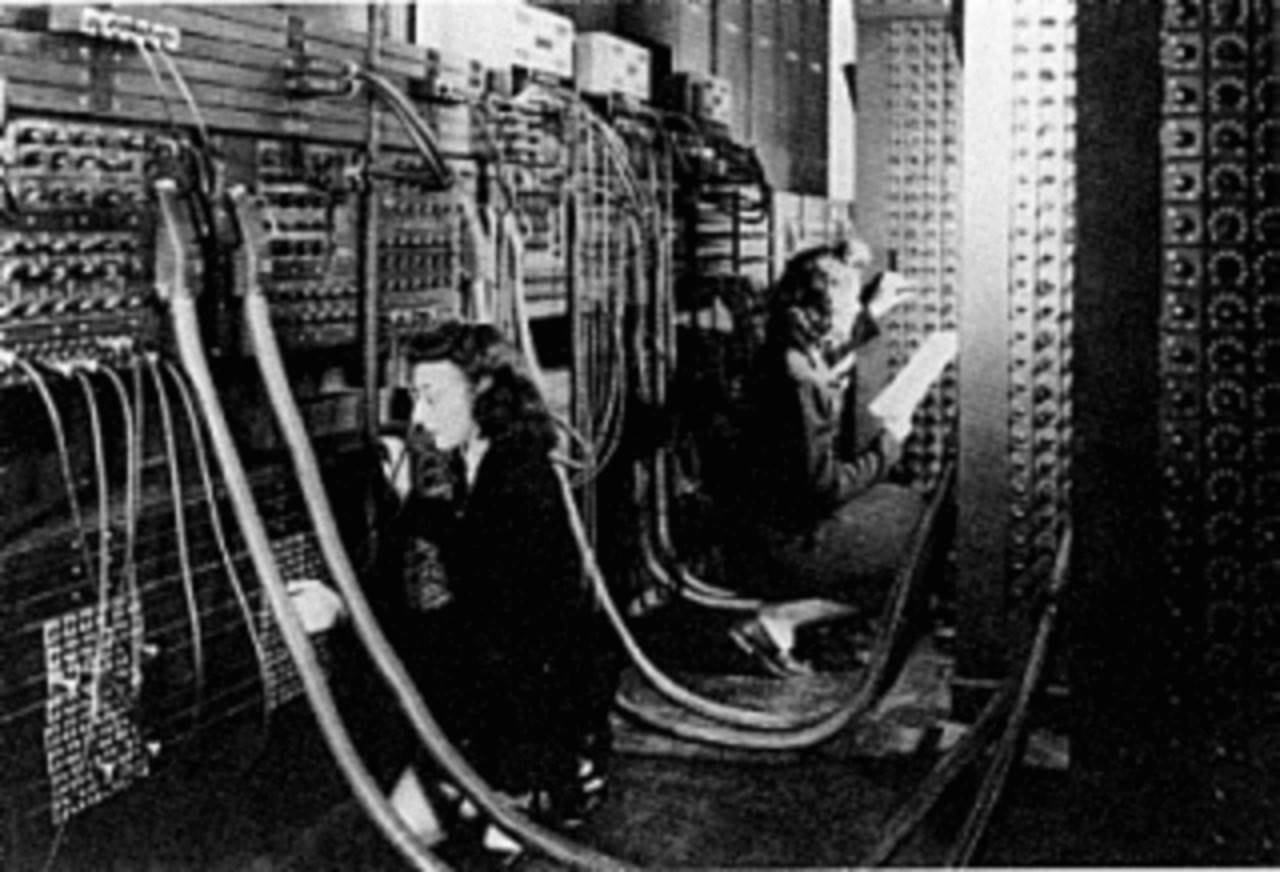
\includegraphics[height=7.5 cm]{PLOTS/eniac-3.jpg}}
\end{onlyenv}

\begin{onlyenv}<4->
\vspace{-7.5 cm}
\mbox{\hspace{2.75 cm}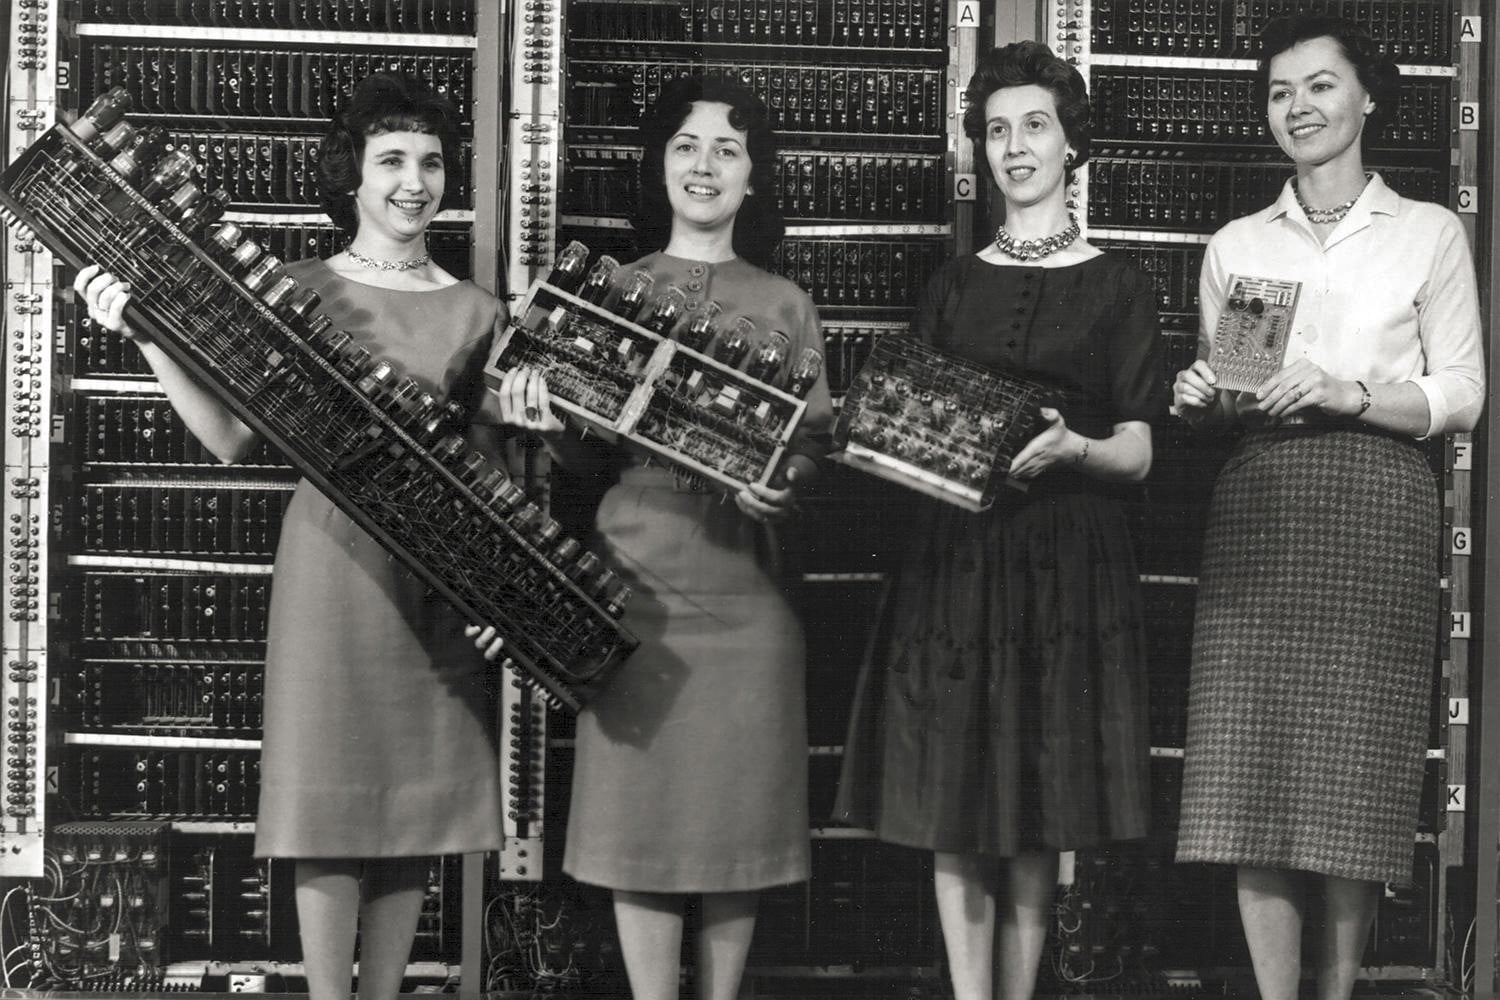
\includegraphics[height=7.5 cm]{PLOTS/eniac-4.jpg}}

\vspace{-2 cm}
\begin{center}
\hspace{3.75 cm}\textcolor{yellow}{\bf Worth mentioning: all 6 of}

\hspace{3.75 cm}\textcolor{yellow}{\bf ENIAC's programmers were women}
\end{center}
\end{onlyenv}
\end{frame}

\end{document}

%% Experimental particle physics is an intensely computational field of science. In fact, particle physicists were arguably the first non-secret (non-cryptography) users of digital computers, and have been pushing the boundaries of pattern recognition and throughput ever since. For decades, our unique needs justified custom software at all levels of the stack, maintained "in-house" by physicists, but the situation changed in the 21st century. Machine learning and analysis of web-scale datasets (i.e. "Big Data") has become an industry on its own, under the catch-all name "data science." Physicists are responding by adopting data science toolsets and methodologies, integrating them with traditional physics software, though the process is ongoing and differs in degree across physics groups. 

%% This talk will present a big picture of how experimental particle physicists have used data analysis software in the past 75 years, how our needs have dictated a choice of programming languages and toolkits, and how those choices are changing. We'll see how pattern recognition evolved from semi-automated to algorithmic to machine learning, how programming languages transitioned from Fortran to C++ to include a significant mix of Python, and how software was organized from site-custom solutions to standard packages like CERNLIB and ROOT to also include a mix of data science tools. Finally, these choices are not purely technical: communities form around software tools, and integrating toolsets integrates physicists with the larger world.

% "neural" and (publication_info.cnum:C85-06-25 or publication_info.cnum:C87-02-02.2 or publication_info.cnum:C89-04-10 or publication_info.cnum:C90-04-09 or publication_info.cnum:C91-03-11 or publication_info.cnum:C92-09-21 or publication_info.cnum:C94-04-21 or publication_info.cnum:C95-09-18 or publication_info.cnum:C97-04-07 or publication_info.cnum:C98-08-31 or publication_info.cnum:C00-02-07 or publication_info.cnum:C01-09-03.1 or publication_info.cnum:C03-03-24.1 or publication_info.cnum:C04-09-27 or publication_info.cnum:C06-02-13 or publication_info.cnum:C07-09-02.1 or publication_info.cnum:C09-03-21 or publication_info.cnum:C10-10-18.4 or publication_info.cnum:C12-05-21.3 or publication_info.cnum:C13-10-14.1 or publication_info.cnum:C15-04-13 or publication_info.cnum:C16-10-14 or publication_info.cnum:C18-07-09.6 or publication_info.cnum:C19-11-04 or publication_info.cnum:C21-05-17.1)

% curl -s 'https://inspirehep.net/api/literature?sort=mostrecent&size=25&page=1&q=%28publication_info.cnum%3AC85-06-25%20or%20publication_info.cnum%3AC87-02-02.2%20or%20publication_info.cnum%3AC89-04-10%20or%20publication_info.cnum%3AC90-04-09%20or%20publication_info.cnum%3AC91-03-11%20or%20publication_info.cnum%3AC92-09-21%20or%20publication_info.cnum%3AC94-04-21%20or%20publication_info.cnum%3AC95-09-18%20or%20publication_info.cnum%3AC97-04-07%20or%20publication_info.cnum%3AC98-08-31%20or%20publication_info.cnum%3AC00-02-07%20or%20publication_info.cnum%3AC01-09-03.1%20or%20publication_info.cnum%3AC03-03-24.1%20or%20publication_info.cnum%3AC04-09-27%20or%20publication_info.cnum%3AC06-02-13%20or%20publication_info.cnum%3AC07-09-02.1%20or%20publication_info.cnum%3AC09-03-21%20or%20publication_info.cnum%3AC10-10-18.4%20or%20publication_info.cnum%3AC12-05-21.3%20or%20publication_info.cnum%3AC13-10-14.1%20or%20publication_info.cnum%3AC15-04-13%20or%20publication_info.cnum%3AC16-10-14%20or%20publication_info.cnum%3AC18-07-09.6%20or%20publication_info.cnum%3AC19-11-04%20or%20publication_info.cnum%3AC21-05-17.1%29' 2>&1 > all-chep-papers.json

%% {
%%     "C85-06-25": 1,
%%     "C87-02-02.2": 2,
%%     "C89-04-10": 3,
%%     "C90-04-09": 4,
%%     "C91-03-11": 5,
%%     "C92-09-21": 6,
%%     "C94-04-21": 7,
%%     "C95-09-18": 8,
%%     "C97-04-07": 9,
%%     "C98-08-31": 10,
%%     "C00-02-07": 11,
%%     "C01-09-03.1": 12,
%%     "C03-03-24.1": 13,
%%     "C04-09-27": 14,
%%     "C06-02-13": 15,
%%     "C07-09-02.1": 16,
%%     "C09-03-21": 17,
%%     "C10-10-18.4": 18,
%%     "C12-05-21.3": 19,
%%     "C13-10-14.1": 20,
%%     "C15-04-13": 21,
%%     "C16-10-14": 22,
%%     "C18-07-09.6": 23,
%%     "C19-11-04": 24,
%%     "C21-05-17.1": 25,
%% }

% 2028 HL-LHC LHCb: https://iopscience.iop.org/article/10.1088/1742-6596/706/2/022002
% 20,000-100,000 events per second
% but really just 20,000: https://cds.cern.ch/record/1701361/files/LHCB-TDR-016.pdf

% 2028 HL-LHC ATLAS: https://cds.cern.ch/record/2285584
% 10,000 events per second

% 2028 HL-LHC CMS: https://cds.cern.ch/record/2020886
% 5000 to 7500 events per second

% 2018 ATLAS: https://cds.cern.ch/record/2725146
% 1200 events per second

% 2017 CMS: http://cds.cern.ch/record/2297540
% 1000 events per second

% ATLAS fact sheet: https://cds.cern.ch/record/1457044/files/ATLAS%20fact%20sheet.pdf
% says 1000 million events recorded per year, from 200 events per second (which would be 6000 million/year, but close enough)

% CMS Run I: https://cms.cern/detector/triggering-and-data-acquisition
% says 100 events per second: ~3000 million events per year

% 2012 LHCb: https://inspirehep.net/literature/1211038
% says 3000 events per second: 90,000 million events per year
% LHCb TDR (http://cds.cern.ch/record/630828) says 200 events per second

% 2009 D0 run II: https://inspirehep.net/literature/812698
% 50-100 events per second

% 1988 CDF run I: https://inspirehep.net/literature/262056
% 20-30 events per second

% 1982 UA1: https://inspirehep.net/literature/176681
% says 10 events per second (limited by tape): 300 million per year

%%% Madeleine Isenberg's scanner salary in 1962: $1.75/hour, over the $1/hour minimum wage; would be worth $15.50/hour today.
